\documentclass{article}
\usepackage[utf8]{inputenc}
\usepackage{amsmath}
\usepackage[margin=1in]{geometry}
\usepackage{caption}
\usepackage{subcaption}
\usepackage{graphicx}
\usepackage{biblatex} 
\addbibresource{library.bib}

\title{NE8 Lecture 1: The neutron transport equation}
\author{Paul Cosgrove}
\date{September 2022}

\begin{document}

\maketitle

\section{Introduction to the course}

Nuclear reactors are driven by energy released from the migration and multiplication of neutrons. This field is often referred to as neutronics. Analytic results of simplified problems (e.g., from NE1) are useful for obtaining some intuitions about neutronics, but numerical approaches are invariably required when it comes to practical reactor design.

This course will cover:
\begin{itemize}
    \item The basic theory of neutron transport
    \item The difficulties of solving the neutron transport equation
    \item The derivation of the neutron diffusion equation
    \item Power iteration: the most common algorithm for solving neutronics eigenvalue equations
    \item Common approaches to discretising the neutron transport equation in space and angle
    \item The `transport sweep', the most popular algorithm for solving industrial neutron transport problems
    \item A brief introduction to treating energy discretisation
    \item Lattice physics -- or how multi-group cross sections are produced for core simulators
    \item An introduction to the Monte Carlo method for neutron transport
\end{itemize}
These will be taught across eight lectures and four workshops, alternating each week, where the workshops introduce a new piece of coursework. Each workshop also has a `help session' later that week (we can negotiate a bit more on the timings...). The four pieces of coursework are:
\begin{itemize}
    \item Numerical solution of the neutron diffusion equation
    \item Numerical solution of the discrete ordinates form of the neutron transport equation
    \item Using the WIMS industrial lattice physics code
    \item Using the Serpent industrial Monte Carlo code
\end{itemize}
The former two pieces of coursework will have you writing your own MATLAB/Python/etc.~code to solve very basic neutronics problems. The latter two pieces will introduce you to industrial codes and use them to realistically explore reactor physics.

I must emphasise: assessment is through \textbf{writing and using codes, and explaining their results}. Assessment is \textbf{not through maths or solving partial differential equations}. This module does contain plenty of maths in the background, but only to show you how and why we use computers to solve neutronics problems -- none of your understanding of the maths is directly assessed.

\section{Neutron transport}

\subsection{The basics}
Our goal is to understand how neutrons move across space and interact with matter. We do so because we want to know the various rates at which nuclear reactions occur across our reactor.

Fundamentally, we want to obtain $n(\mathbf{r},\mathbf{\Omega},E,t)$. This is the \textbf{angular neutron density} with units of neutrons/cm$^3$/steradian/MeV, which tells us \textbf{the expected number of neutrons at a point in phase space}. The independent variables are $\mathbf{r}$, the position vector (where the neutrons are in space), $\mathbf{\Omega}$, the direction unit vector (where the neutrons are pointing, or the direction in which they are travelling), $E$, the neutron energy, and $t$, the point in time. Some authors combine $\mathbf{\Omega}$ and $E$ into one variable to give the neutron velocity vector, $\mathbf{v}$, with a magnitude $v = |\mathbf{v}|$, but this is usually less convenient in reactor physics. This is visualised in Fig.~\ref{fig:phase_space}. Note that I emphasise the \textbf{expected} number of neutrons. This is because neutrons do behave in a stochastic manner thanks to quantum physics and the number of neutrons about a point in phase space will fluctuate. However, if we have many neutrons (like in a reactor) then the fluctuations around this expected number should be small -- if that were not the case then our analysis would become much more complicated.

\begin{figure}[h]
     \centering
     \begin{subfigure}{0.45\textwidth}
         \centering
         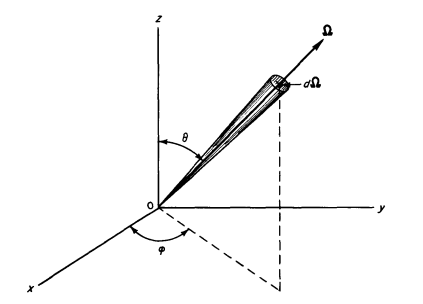
\includegraphics[width=1\textwidth]{angular.png}
         \caption{Angular variables. $\varphi$ is referred to as the azimuthal angle, while $\theta$ is the polar angle. Note that $\int_{4\pi}\mathrm{d}\Omega = \int^{2\pi}_0\mathrm{d}\varphi\int^{\pi}_{0}\sin(\theta)\mathrm{d}\theta = 4\pi$}
     \end{subfigure}
     \begin{subfigure}{0.45\textwidth}
         \centering
         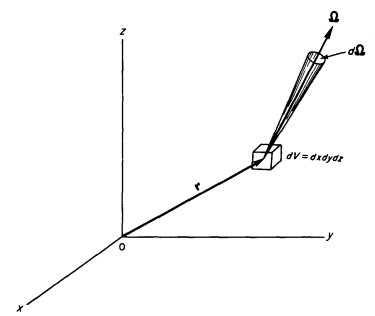
\includegraphics[width=1\textwidth]{volume.png}
         \caption{Spatial variables}
     \end{subfigure}
        \caption{Geometric phase space variables in neutron transport~\cite{Bell}}
        \label{fig:phase_space}
\end{figure}

Why are these the important independent variables? Well, space, energy, and time are hopefully fairly obvious by now. Due to things like leakage, or the separation of fuel and moderator, the number of neutrons will vary across space. Likewise, we all know how cross sections vary dramatically in energy, and therefore at energies close to resonances, for example, there will be fewer neutrons than about 1 MeV, where neutrons tend to be born. Finally, reactor physicists are naturally interested in the transient behaviour of nuclear reactors, so time evolution is of some concern. That said, you will soon see that this can often be avoided because much of our reactor analysis occurs at their critical state or during very slow transients.

The less familiar variable is $\mathbf{\Omega} = \cos(\varphi)\sin(\theta)\mathbf{i} + \sin(\varphi)\sin(\theta)\mathbf{j} + \cos(\theta)\mathbf{k}$, the direction vector in which neutrons travel. This variable appears because neutrons can `stream' long distances in a given direction without colliding. Noting that neutrons and photons behave similarly, if you had an X-ray machine, how would diffusive photons behave? How does this differ from actual X-ray machines?

In principle there are other variables that could also be included (like the neutron's spin direction), but these are not very important for reactor physics applications.

You may also recall from previous courses that the neutron density by itself is not often useful. We care about \textbf{the rates of neutron interactions with matter} which are determined by the neutron density multiplied by the neutron speed and the local neutron cross section. Therefore it makes the final equations a bit more compact to define a new quantity, the neutron angular flux:
\begin{equation}
    \psi(\mathbf{r},\mathbf{\Omega},E,t) = vn\; \mathrm{.}
\end{equation} 
Usually we care about neutrons travelling in all directions about some point in space, energy, and time. Therefore, we also define the familiar neutron scalar flux by integrating the angular flux over the unit sphere:
\begin{equation}
    \phi(\mathbf{r},E,t) = \int_{4\pi}\mathrm{d}\Omega \psi \;\mathrm{.} 
\end{equation}
We are often interested in the net number of neutrons travelling in a given direction -- the familiar neutron current. This is defined as:
\begin{equation}
    \mathbf{J}(\mathbf{r},E,t) = \int_{4\pi}\mathrm{d}\Omega\mathbf{\Omega}\psi\;\mathrm{.}
\end{equation}
%Note that the differential in the integration is a scalar, not a vector.
This should also be familiar, but as a brief refresher, the rate at which reaction $x$ occurs over some volume of space, $V$, and in the energy range $E_1$ to $E_2$ at a fixed point in time is:
\begin{equation}\label{eq:reaction}
    R_x(t) = \int_V \mathrm{d}V \int^{E_2}_{E_1} \mathrm{d}E\; \Sigma_x(\mathbf{r},E) \phi(\mathbf{r},E,t) \;\mathrm{,}
\end{equation}
where $\Sigma_x$ is the macroscopic cross section for reaction type $x$.

With all of these quantities defined, we can derive an equation which should accurately describe the behaviour of neutrons in reactors.

\subsection{The transport equation}

We want to obtain the dynamic balance equation for neutrons travelling at energies $\pm \mathrm{d}E$ about $E$, at angles $\pm \mathrm{d}\mathbf{\Omega}$ about $\mathbf{\Omega}$ inside an arbitrary volume $V$. Coarsely this balance can be written as:
\begin{equation}\label{eq:balance_words}
    \textrm{Change in neutrons over time} = \textrm{Addition of neutrons} - \textrm{Loss of neutrons}\;\mathrm{.} 
\end{equation}
We can break this down by considering the sources and sinks of neutrons.

\subsubsection{Fission source}

You hopefully know that neutrons can emerge from neutron-induced reactions. Given Eq.~\eqref{eq:reaction} and neglecting time for now, the rate of all fission reactions in some volume $V$ is:
\begin{equation}
    \textrm{Fission rate} = \int_V \mathrm{d}V\int^\infty_0 \mathrm{d}E \;\Sigma_\mathrm{f}(\mathbf{r},E)\phi(\mathbf{r},E)\;\mathrm{,}
\end{equation}
where $\Sigma_\mathrm{f}$ is the macroscopic fission cross section. Fission produces multiple neutrons, so to work out the source we must include the average number of neutrons per fission, $\bar{\nu}(\mathbf{r},E)$, which depends on the material undergoing fission and the energy of the incoming neutrons -- we usually combine this with $\Sigma_\mathrm{f}$ and refer to the `fission production cross section', $\bar{\nu}\Sigma_\mathrm{f}$. Neutrons born in fission are produced with a particular spectrum/energy distribution, which we denote as $\chi(E)$. These neutrons are also born with an isotropic distribution to a very good approximation. Therefore, the number of neutrons produced at energy $E$, pointing in direction $\mathbf{\Omega}$ inside the volume $V$ is:
\begin{equation}\label{eq:fission production}
\begin{split}
    \textrm{Fission neutron production rate} = &\\
    \frac{\chi(E)}{4\pi}\int_V \mathrm{d}V\int^\infty_0 \mathrm{d}E' \;\bar{\nu}\Sigma_\mathrm{f}(\mathbf{r},E')\phi(\mathbf{r},E')\;\mathrm{.}
\end{split}
\end{equation}
For now, this will be kept simple, but we could complicate fission by including delayed neutrons. If we did, Eq.~\eqref{eq:fission production} would have a $1-\beta$ multiplier (where $\beta$ is the delayed neutron fraction), $\chi$ would be the \textbf{prompt} neutron spectrum, and we would have another term accounting for the production of delayed neutrons through precursor decay.

\subsubsection{Scattering source}

We can treat scattering similarly to fission, but I should emphasise: \textbf{neutrons do not generally scatter isotropically!} This causes many headaches. To hide this pain, we devise what is called the `double differential scattering cross section', $\Sigma_\mathrm{s}\left(\mathbf{r},\mathbf{\Omega}'\rightarrow\mathbf{\Omega},E'\rightarrow E\right)$. This is to say that there is a cross section which describes the distribution of how incoming neutrons' energies and angles ($E',\mathbf{\Omega}'$) are transformed into outgoing energies and angles ($E,\mathbf{\Omega}$). As such, we can write the rate at which neutrons are produced from scattering at energy $E$, pointing in direction $\mathbf{\Omega}$ inside the volume $V$ as:
\begin{equation}
\begin{split}
    \textrm{Scattered neutron production rate} = &\\
    \int_V \mathrm{d}V\int^\infty_0 \mathrm{d}E'\int_{4\pi}\mathrm{d}{\Omega}' \;\Sigma_\mathrm{s}\left(\mathbf{r},\mathbf{\Omega}'\rightarrow\mathbf{\Omega},E'\rightarrow E\right)\psi(\mathbf{r},\mathbf{\Omega}',E')\;\mathrm{.}
\end{split}
\end{equation}
This term can also include multiplication by accounting for (n,2n), (n,3n), etc.~reactions.

\subsubsection{Inhomogeneous sources}
We can also have other sources of neutrons in a reactor which don't depend on the flux of neutrons. This might be an initiator from an ($\alpha$,n) source, spontaneous fissions of isotopes present, or even neutrons produced from cosmic radiation. Often these sources are quite small in power reactor problems and tend to be neglected. Typically this source is written as $Q(\mathbf{r},\mathbf{\Omega},E)$.

\subsubsection{Loss through collision}
Neutrons in the volume $V$, travelling in the direction $\mathbf{\Omega}$ at energy $E$ can be lost on collision with a material -- either through absorption or scattering. This rate is given simply as:
\begin{equation}
    \textrm{Collision loss rate} = \int_V \mathrm{d}V\; \Sigma_\mathrm{t}(\mathbf{r},E) \psi (\mathbf{r},\mathbf{\Omega},E)\;\mathrm{,}
\end{equation}
where $\Sigma_\mathrm{t}$ is the total cross section.

\subsubsection{Loss through leakage}

The volume $V$ that we are considering is enclosed by a surface $S$ -- this is illustrated in Fig.~\ref{fig:surface}. We can use this to calculate the number of neutrons entering or exiting through this surface. A surface element of $S$ is given by $\mathrm{d}\mathbf{S}$ (with the vector component pointing out of the surface). The number of neutrons leaking out of $S$ per second is then given by (remembering $\psi = vn$):
\begin{equation}
    \textrm{Leakage rate across $S$} = \int_S \mathrm{d}\mathbf{S}\cdot\mathbf{\Omega}\psi(\mathbf{r},\mathbf{\Omega},E)\;\mathrm{.}
\end{equation}
We can use the divergence theorem to transform this into a volume integral:
\begin{equation}
    \int_S \mathrm{d}\mathbf{S}\cdot\mathbf{\Omega}\psi = \int_V \mathrm{d}V\; \nabla\cdot\mathbf{\Omega}\psi\;\mathrm{.}
\end{equation}
Finally, by a vector identity, we can exchange the order of $\nabla$ and $\mathbf{\Omega}$ to give:
\begin{equation}
    \textrm{Net leakage rate out of $V$} =\int_V \mathrm{d}V\; \mathbf{\Omega}\cdot\nabla\psi\;\mathrm{.}
\end{equation}

\begin{figure}[h]
        \centering
        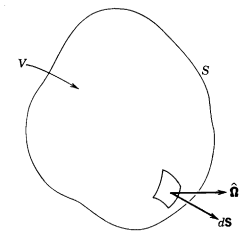
\includegraphics[width=0.4\textwidth]{surface_leakage.png}
        \caption{Illustration of a bounding surface and leakage from a surface element~\cite{Duderstadt}}
        \label{fig:surface}
\end{figure}

\subsubsection{Putting it all together}

Rewriting Eq.~\eqref{eq:balance_words} symbolically, we have:
\begin{equation}
\begin{split}
    &\int_V\mathrm{d}V\Bigg[\frac{\partial n}{\partial t}  +\mathbf{\Omega}\cdot\nabla\psi + \Sigma_\mathrm{t}\psi
    -\frac{\chi(E)}{4\pi}\int^\infty_0 \mathrm{d}E' \;\bar{\nu}\Sigma_\mathrm{f}(\mathbf{r},E')\phi(\mathbf{r},E',t) \\
    &-\int^\infty_0 \mathrm{d}E'\int_{4\pi}\mathrm{d}{\Omega}' \;\Sigma_\mathrm{s}\left(\mathbf{r},\mathbf{\Omega}'\rightarrow\mathbf{\Omega},E'\rightarrow E\right)\psi(\mathbf{r},\mathbf{\Omega}',E',t)\Bigg] = 0\;\mathrm{.}
\end{split}
\end{equation}
We note that the volume integral is performed on all terms over an arbitrary volume and so can be removed. Also, we can rewrite the time derivative to be more convenient, giving:
\begin{equation}
\begin{split}
    &\frac{1}{v}\frac{\partial \psi}{\partial t}  +\mathbf{\Omega}\cdot\nabla\psi + \Sigma_\mathrm{t}\psi
    =\frac{\chi(E)}{4\pi}\int^\infty_0 \mathrm{d}E' \;\bar{\nu}\Sigma_\mathrm{f}(\mathbf{r},E')\phi(\mathbf{r},E',t) \\
    &+\int^\infty_0 \mathrm{d}E'\int_{4\pi}\mathrm{d}{\Omega}' \;\Sigma_\mathrm{s}\left(\mathbf{r},\mathbf{\Omega}'\rightarrow\mathbf{\Omega},E'\rightarrow E\right)\psi(\mathbf{r},\mathbf{\Omega}',E',t)\;\mathrm{.}
    \end{split}
\end{equation}
This is the \textbf{time-dependent neutron transport equation} (without delayed neutrons and inhomogeneous sources).

Implicitly, we have made several assumptions in arriving at this equation. These include:
\begin{itemize}
    \item Neglecting neutron-neutron interactions (~10$^{11}$ n/cm$^3$ in thermal reactors versus ~10$^{22}$ atoms/cm$^3$ in solids)
    \item Neglecting gravity
    \item Neglecting relativistic effects (fast neutrons travel at $~0.04c$)
    \item Assuming neutrons are point particles (thermal neutron wavelength is $~2$\AA)
    \item Assuming collisions occur instantaneously
    \item Neglecting motion of the medium
    \item Neglecting neutron decay (they have a half-life of about 12 minutes)
    \item Neglecting other particles producing neutrons (e.g., photofission)
    \item Assume a large population of neutrons (so fluctuations driven by the stochastic behaviour of individual neutrons are small)
\end{itemize}
And more! However, these are all good assumptions for nuclear reactor physics but can be relaxed with more complication and eventual computational effort. But we have one more simplification to make life easier for reactor physicists...

\section{The k-eigenvalue form of the transport equation}

Time-dependent problems are very difficult to solve and we would rather avoid this if we can. Nuclear reactors are often static, or change very slowly in time. This is because reactors tend to operate about criticality or $k\approx1$. In a system with fissile material, $k$ can be used to scale the rate at which fission occurs, increasing or decreasing it until a steady state can be reached -- this would zero the $\frac{\partial \psi}{\partial t}$ term in the transport equation, making it much easier to solve. The value of $k$ for which this occurs is known as $k_\mathrm{eff}$. Hence, the transport equation becomes:
\begin{equation}\label{eq:NTE}
\begin{split}
    &\mathbf{\Omega}\cdot\nabla\psi + \Sigma_\mathrm{t}\psi
    =\frac{\chi(E)}{4\pi k_\mathrm{eff}}\int^\infty_0 \mathrm{d}E' \;\bar{\nu}\Sigma_\mathrm{f}(\mathbf{r},E')\phi(\mathbf{r},E') \\
    &+\int^\infty_0 \mathrm{d}E'\int_{4\pi}\mathrm{d}{\Omega}' \;\Sigma_\mathrm{s}\left(\mathbf{r},\mathbf{\Omega}'\rightarrow\mathbf{\Omega},E'\rightarrow E\right)\psi(\mathbf{r},\mathbf{\Omega}',E')\;\mathrm{.}
    \end{split}
\end{equation}
This is the integro-differential neutron transport equation with which most of reactor physics (and all of this course) is concerned. We will spend the rest of NE8 simplifying it so that a computer can solve it to give us fluxes, reaction rates, and the value of $k_\mathrm{eff}$.

One thing to note is that $\chi$ in this equation is not the same as that in the time-dependent equation -- this is because it must account for neutrons which are produced by precusors as well (which tend to be more thermal). Also note, this equation requires boundary conditions to be able to be solved. Usually we choose these to be reflective (neutrons bounce back from walls), periodic (neutrons re-enter from the opposite wall), or vacuum (neutrons disappear and never return). We'll talk more about this later.

\section{Challenges with the neutron transport equation}

Eq.~\eqref{eq:NTE} is in some senses very simple: it's an eigenvalue problem, which is very common in computational physics, there are no non-linear terms (like, say, in fluid dynamics), and it is time-independent. Unfortunately, the transport equation is also 6-dimensional and varies strongly in each of those dimensions, requiring very fine discretisation (compromising a computer's memory) or approximation (compromising solution accuracy). Typically we use both strategies in some combination.

Fig.~\ref{fig:thermal_flux} shows the thermal neutron flux across two fuel assemblies adjacent to a water reflector. One of these assemblies is UOX, one is MOX, and both have several guide tubes. Can you identify which is which? Flux can vary substantially across a pin and between adjacent pins. Estimating it correctly is important to identifying hot spots and accurately predicting how fuel will burn over its life. 

\begin{figure}[h]
        \centering
        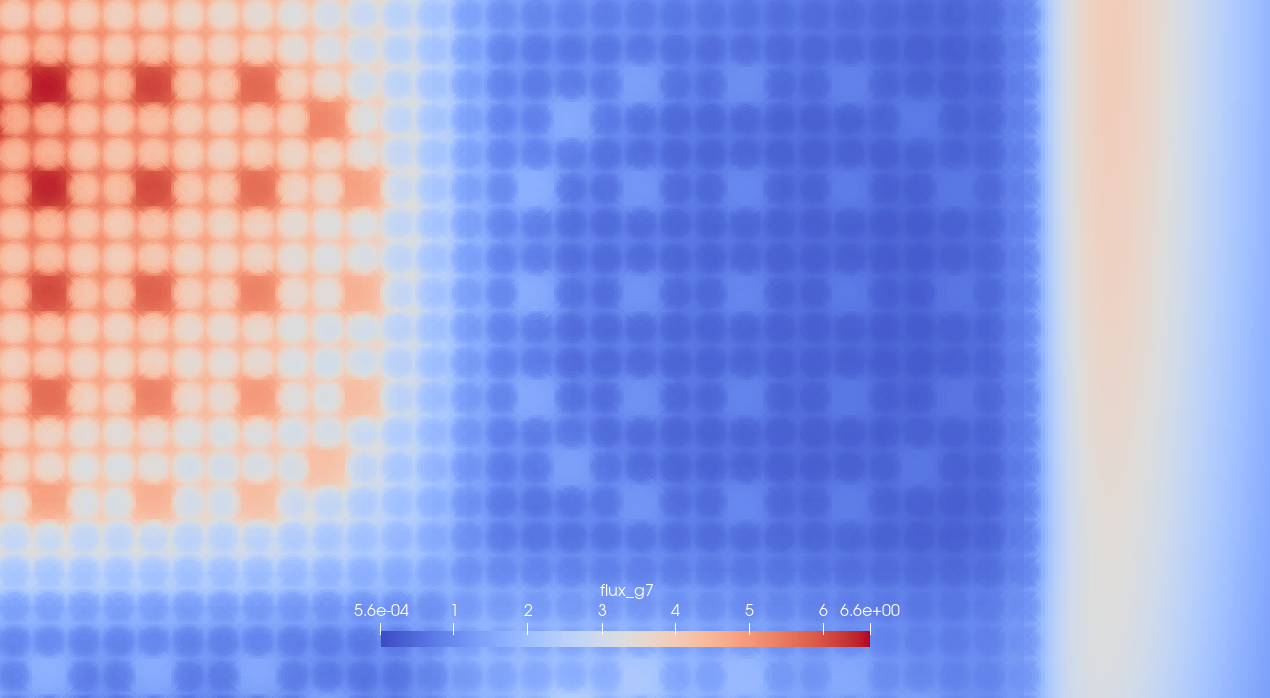
\includegraphics[width=0.6\textwidth]{thermal_flux.png}
        \caption{Thermal flux across part of a reactor}
        \label{fig:thermal_flux}
\end{figure}

Due to the nature of cross sections, nuclear reaction rates vary tremendously in energy. This can be seen in Fig.~\ref{fig:energy_variation} which shows the familiar phenomenon of energy self-shielding -- note the logarithmic axes!

\begin{figure}[h]
     \centering
     \begin{subfigure}{0.45\textwidth}
         \centering
         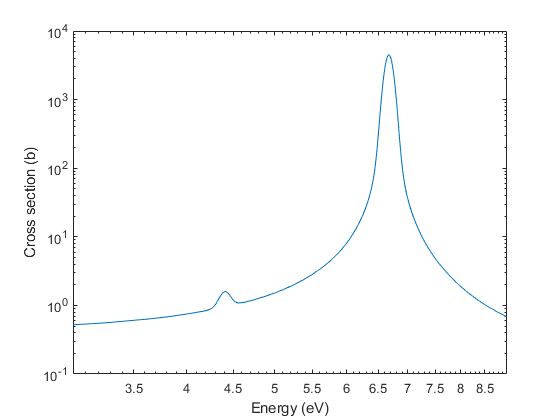
\includegraphics[width=0.9\textwidth]{cross_section_238.png}
         \caption{$^{238}$U capture cross section about a resonance}
     \end{subfigure}
     \begin{subfigure}{0.45\textwidth}
         \centering
         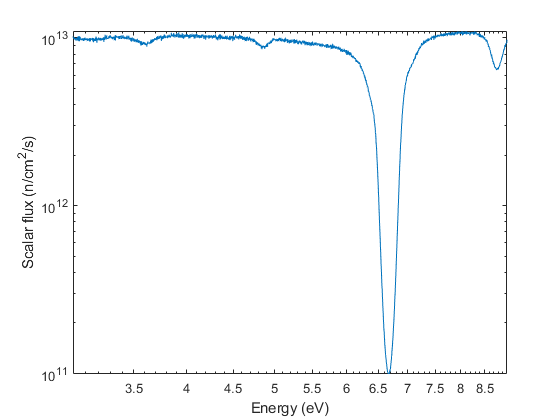
\includegraphics[width=0.9\textwidth]{scalar_flux_238.png}
         \caption{Scalar flux in fuel around $^{238}$U's largest resonance}
     \end{subfigure}
        \caption{The challenges of energy discretisation in neutronics}
        \label{fig:energy_variation}
\end{figure}

Finally, $\psi$ is extremely anisotropic in the vicinity of material boundaries or where localised sources are present. An example of this is shown in Fig.~\ref{fig:angular_flux}, where the fast angular flux is shown about a point in a reactor pin cell lattice -- note the discontinuities which would require fine angular discretisation to resolve. For context, neutron diffusion assumes that flux is only linearly anisotropic.

\begin{figure}[h]
        \centering
        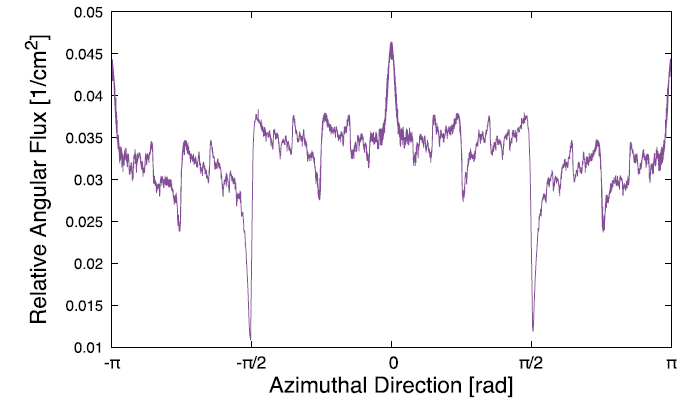
\includegraphics[width=0.6\textwidth]{angular_flux.png}
        \caption{Fast neutron angular flux in a 2D pin cell lattice~\cite{Tramm2017}}
        \label{fig:angular_flux}
\end{figure}

\section{Simplifying the transport equation}

We want to simplify the transport equation further before doing anything with it. We will do so by removing energy dependence and anisotropic scattering. Neither of these simplifications are necessary, but they make understanding things (and coding solvers) a lot simpler.

\subsection{Multi-group representation and removing energy dependence}
Cross sections vary continuously in energy. When discretising the transport equation, we approximate this by saying they are piecewise constant over given energy ranges, known as energy `groups'. Instead of having $\Sigma_x(E)$ we have $\Sigma^g_x$ where $g$ is the energy group containing energy $E$. To do this we have to make group-average cross sections and tend to do this as:
\begin{equation}
    \Sigma^g_x = \frac{\int^{E_{g-1}}_{E_g}\mathrm{d}E\; \Sigma_x(E)\phi(E)}{\int^{E_{g-1}}_{E_g}\mathrm{d}E\; \phi(E)}\;\mathrm{,}
\end{equation}
where $E_{g-1}$ and $E_g$ are the upper and lower energy bounds of energy group $g$. We'll talk about why and how we take this approach another day. We can plug these cross sections into the transport equation and then integrate it over energy to get:
\begin{equation}
    \begin{split}
 &\mathbf{\Omega}\cdot\nabla\psi^g + \Sigma^g_\mathrm{t}\psi^g
    =\frac{\chi^g}{4\pi k_\mathrm{eff}}\sum_{g'} \;\bar{\nu}\Sigma^{g'}_\mathrm{f}\phi^{g'} \\
    &+\sum_{g'}\int_{4\pi}\mathrm{d}{\Omega}' \;\Sigma^{g'\rightarrow g}_\mathrm{s}\left(\mathbf{\Omega}'\rightarrow\mathbf{\Omega}\right)\psi^{g'}\;\mathrm{,}
    \end{split}
\end{equation}
where the $g$ and $g'$ superscripts denote given energy groups and $\psi^g$ and $\phi^g$ are the angular/scalar fluxes integrated over energy group $g$. If we have $G$ energy groups in total, we go from having a single neutron transport equation in continuous energy to having $G$ transport equations with discrete energies coupled together by scattering and fission.

In the extreme case we might choose to have only a single energy group ($G=1$). This is not very good if we want to do a reactor simulation, but it makes manipulating the equations much easier. This results in the monoenergetic transport equation:
\begin{equation}
    \begin{split}
 \mathbf{\Omega}\cdot\nabla\psi + \Sigma_\mathrm{t}\psi
    =\frac{1}{4\pi}\frac{\bar{\nu}\Sigma_\mathrm{f}}{ k_\mathrm{eff}}\phi +\int_{4\pi}\mathrm{d}{\Omega}' \;\Sigma_\mathrm{s}\left(\mathbf{\Omega}'\rightarrow\mathbf{\Omega}\right)\psi\;\mathrm{,}
    \end{split}
\end{equation}
where $\psi$, $\phi$, and all cross sections no longer vary in energy.

\subsection{Anisotropic scattering}

The scattering kernel, $\Sigma_\mathrm{s}\left(\mathbf{r},\mathbf{\Omega}'\rightarrow\mathbf{\Omega}\right)$ can be separated into a cross section component and a scattering distribution component:
\begin{equation}
\Sigma_\mathrm{s}\left(\mathbf{r},\mathbf{\Omega}'\rightarrow\mathbf{\Omega}\right) = \Sigma_\mathrm{s}(\mathbf{r})f(\mathbf{\Omega}'\rightarrow\mathbf{\Omega})\;\mathrm{,}
\end{equation}
where $\Sigma_\mathrm{s}$ is the scattering cross section and $f$ is the outgoing angle (and generally energy) distribution given an incoming angle (and energy). In most cases of interest, the relationship between incoming and outgoing angles is through their cosine, so that we can write:
\begin{equation}
f(\mathbf{\Omega}'\rightarrow\mathbf{\Omega}) = f(\mathbf{\Omega}'\cdot\mathbf{\Omega})=f(\mu_0)\;\mathrm{,}
\end{equation}
where $\mu_0=\mathbf{\Omega}'\cdot\mathbf{\Omega}$. As this scattering cosine is bounded in the range $[-1,1]$, it is commonly represented as a Legendre polynomial expansion:
\begin{equation}\label{eq:legendre_expansion}
    f(\mu_0) = \sum^\infty_{n=0}\frac{2n+1}{4\pi}f_n P_n(\mu_0)\;\mathrm{,}
\end{equation}
where $P_n(\mu_0)$ is the $n$-th order Legendre polynomial. The first few of these are shown in Fig.~\ref{fig:legendre}. The reason for doing this is simply because it is a relatively compact way to represent these distributions -- not because of any physics or tricks of maths!

\begin{figure}
    \centering
    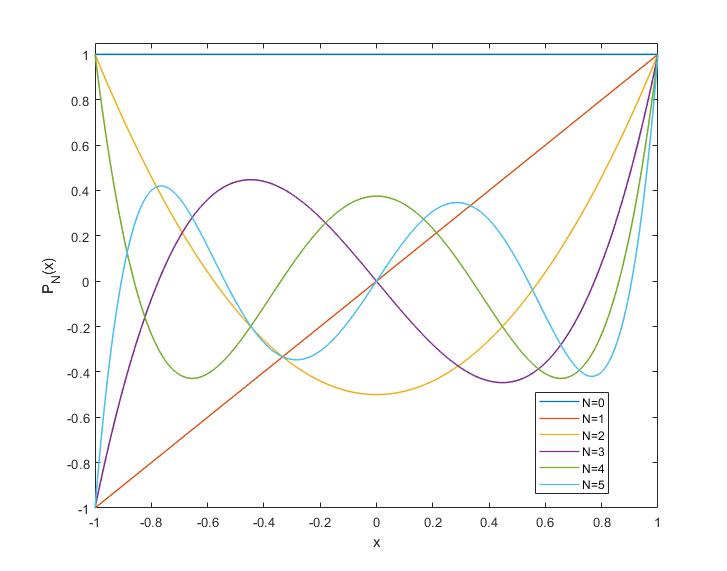
\includegraphics[width=0.6\textwidth]{legendre.png}
    \caption{Plot of the first few Legendre polynomials}
    \label{fig:legendre}
\end{figure}

In reactors, the most prominent scattering anisotropy is due to hydrogen -- this is essentially linearly anisotropic. Therefore, it's not uncommon to truncate to $N=1$, giving:
\begin{equation}\label{eq:linear_anisotropy}
    \begin{split}
 \mathbf{\Omega}\cdot\nabla\psi + \Sigma_\mathrm{t}\psi
    =\frac{1}{4\pi}\frac{\bar{\nu}\Sigma_\mathrm{f}}{ k_\mathrm{eff}}\phi + \frac{1}{4\pi}\int_{4\pi}\mathrm{d}\Omega' \left(\Sigma_{\mathrm{s},0} + 3\left(\mathbf{\Omega}\cdot\mathbf{\Omega}'\right)\Sigma_{\mathrm{s},1}\right)\psi(\mathbf{\Omega}')\;\mathrm{,}
    \end{split}
\end{equation}
where $\Sigma_{\mathrm{s},0}$ and $\Sigma_{\mathrm{s},1}$ are the zeroth and first Legendre moments of the scattering cross section. This means that if we were to represent the scattering kernel as a Legendre series (as in Eq.~\eqref{eq:legendre_expansion}) the coefficients of the first two terms would be $\Sigma_{\mathrm{s},0}$ and $\Sigma_{\mathrm{s},1}$. %This equation is often used in deriving the neutron transport equation. %WTF did mean by this??

We could keep this representation and numerically solve the transport equation with anisotropic scattering, but it can also be approximated away reasonably well in reactor problems by assuming scattering is isotropic and adding a correction term. The means of accurately approximating this is still an ongoing area of research, but the classical approach defines a `transport correction' $\Delta = \Bar{\mu}\Sigma_s$, where $\Bar{\mu}$ is the average neutron scattering cosine in the given material. This is subtracted from both the scattering cross section and the total cross section, giving `transport corrected' cross sections and the Legendre expansion is truncated to 0-th order. As a result, the transport equation can be written more simply as:
\begin{equation}\label{eq:isotropic}
    \begin{split}
 \mathbf{\Omega}\cdot\nabla\psi + \Sigma_\mathrm{tr}\psi
    =\frac{1}{4\pi}\frac{\bar{\nu}\Sigma_\mathrm{f}}{ k_\mathrm{eff}}\phi + \frac{1}{4\pi}\Sigma_\mathrm{s}\phi\;\mathrm{,}
    \end{split}
\end{equation}
where $\Sigma_\mathrm{tr} = \Sigma_t - \Delta$ is commonly known as the transport cross section. This smaller cross section can be thought of as accounting for the forward-peaked scattering that is no longer included in the scattering term. For some reason the scattering cross section does not usually get renamed, despite having $\Delta$ subtracted as well! Accurately calculating this transport correction is extremely non-trivial in the general case and has been known to be a magic factor sitting in the back of industrial lattice physics codes!

In the next lecture we'll manipulate Eq.~\eqref{eq:isotropic} to produce the diffusion equation.

\printbibliography

\end{document}
